%%%%%%%%%%%%%%%%%%%%%%% file template.tex %%%%%%%%%%%%%%%%%%%%%%%%%
%
% This is a general template file for the LaTeX package SVJour3
% for Springer journals.          Springer Heidelberg 2010/09/16
%
% Copy it to a new file with a new name and use it as the basis
% for your article. Delete % signs as needed.
%
% This template includes a few options for different layouts and
% content for various journals. Please consult a previous issue of
% your journal as needed.
%
%%%%%%%%%%%%%%%%%%%%%%%%%%%%%%%%%%%%%%%%%%%%%%%%%%%%%%%%%%%%%%%%%%%
%
% First comes an example EPS file -- just ignore it and
% proceed on the \documentclass line
% your LaTeX will extract the file if required
\begin{filecontents*}{example.eps}
%!PS-Adobe-3.0 EPSF-3.0
%%BoundingBox: 19 19 221 221
%%CreationDate: Mon Sep 29 1997
%%Creator: programmed by hand (JK)
%%EndComments
gsave
newpath
  20 20 moveto
  20 220 lineto
  220 220 lineto
  220 20 lineto
closepath
2 setlinewidth
gsave
  .4 setgray fill
grestore
stroke
grestore
\end{filecontents*}
%
\RequirePackage{fix-cm}
%
\documentclass{svjour3}                     % onecolumn (standard format)
%\documentclass[smallcondensed]{svjour3}     % onecolumn (ditto)
% \documentclass[smallextended]{svjour3}       % onecolumn (second format)
%\documentclass[twocolumn]{svjour3}          % twocolumn
%
\smartqed  % flush right qed marks, e.g. at end of proof
%
\usepackage{graphicx}
%
% \usepackage{mathptmx}      % use Times fonts if available on your TeX system
%
% insert here the call for the packages your document requires
%\usepackage{latexsym}
\usepackage{amsmath}

% etc.
%
% please place your own definitions here and don't use \def but
% \newcommand{}{}
%
% Insert the name of "your journal" with
% \journalname{myjournal}
%
\begin{document}

\title{Investigating exploration for deep reinforcement learning of concentric tube robot control
\thanks{This work is supported by the Wellcome/EPSRC Centre for Interventional and Surgical Sciences (WEISS) (203145Z/16/Z).}
}

%\titlerunning{Short form of title}        % if too long for running head

\author{Keshav Iyengar \and
        George Dwyer \and Danail Stoyanov
}

%\authorrunning{Short form of author list} % if too long for running head

\institute{K. Iyengar \at
              Gower St, Bloomsbury, London WC1E 6BT\\
              \email{keshav.iyengar@ucl.ac.uk} %  \\
%             \emph{Present address:} of F. Author  %  if needed
}

\date{Received: date / Accepted: date}
% The correct dates will be entered by the editor


\maketitle

\begin{abstract}
\leavevmode\newline
\textbf{Purpose} Concentric tube robots are composed of multiple concentric, pre-curved, super-elastic telescopic tubes that are compliant and have a small diameter footprint ideal for minimally invasive surgery. The overall shape can be manipulated by rotating and extending the tubes relative to each other. The interactions between tubes is complex and closed form inverse kinematics are difficult to formulate past trivial tube architectures. A model-free, data driven approach (DDA) such as reinforcement learning would be useful to form the inverse kinematics solution.
\newline
\textbf{Method} Reinforcement learning has a key trade-off problem, exploration versus exploitation and balancing this trade-off is an important step in converging to a control policy. To this end, this work investigates various exploration strategies are investigated for deep deterministic policy gradient with hindsight experience replay with a dominant stiffness concentric tube robot simulation environment. The aim of the study is to determine which, if any, exploration strategies are scalable with respect to number of tubes, an indicator of generality.
\newline
\textbf{Results} The study determines that a zero mean single variate Gaussian noise applied to actions does not explore the workspace in extended joint states. Zero mean multivariate Gaussian of various forms performs much better in exploration of the workspace. Various tube configurations of curvature and relative lengths are tested with the trained model of a given to demonstrate adaptability.
\newline
\textbf{Conclusion} In future works, the found noise process can be applied to variable curvature concentric tube robot models.
\keywords{deep reinforcement learning \and inverse kinematics \and model-free \and policy gradient \and concentric tube robots}
\end{abstract}

\section{Introduction}
\label{intro}
Minimally invasive surgery (MIS) encompasses are large group of techniques that minimize the incision point size in order to reduce healing time and risk of infection. Robotics incorporated with MIS aids the surgeon with precision, vision and ergonomics where traditional MIS is technically challenging because of disassociation of vision and ergonomic factors like monitor placement and operation table height. In some interventions, like those performed with robotic catheters and endoscopes, the robotic devices used are passive along the length and rely on anatomical structures to guide their movement. Any compliance added to the device to limit contact forces with these structures often has the trade-off of reduced tip stiffness detrimental to certain surgical tasks. A greater risk is relying on anatomical structures for guidance can cause damage to surrounding sensitive healthy tissue. Continuum robots are type of robot that have a large number of degrees of freedom distributed along the length of the the robot allowing for tentacle-like motion, advantageous to avoid sensitive structures in the body. Concentric tube robots are a sub-type of continuum robots that use neighboring tube interactions of bending and twisting when rotated and translated to form curvilinear paths. These paths can avoid anatomical structures, be compliant and still offer some dexterity at the tip.
\begin{figure}
  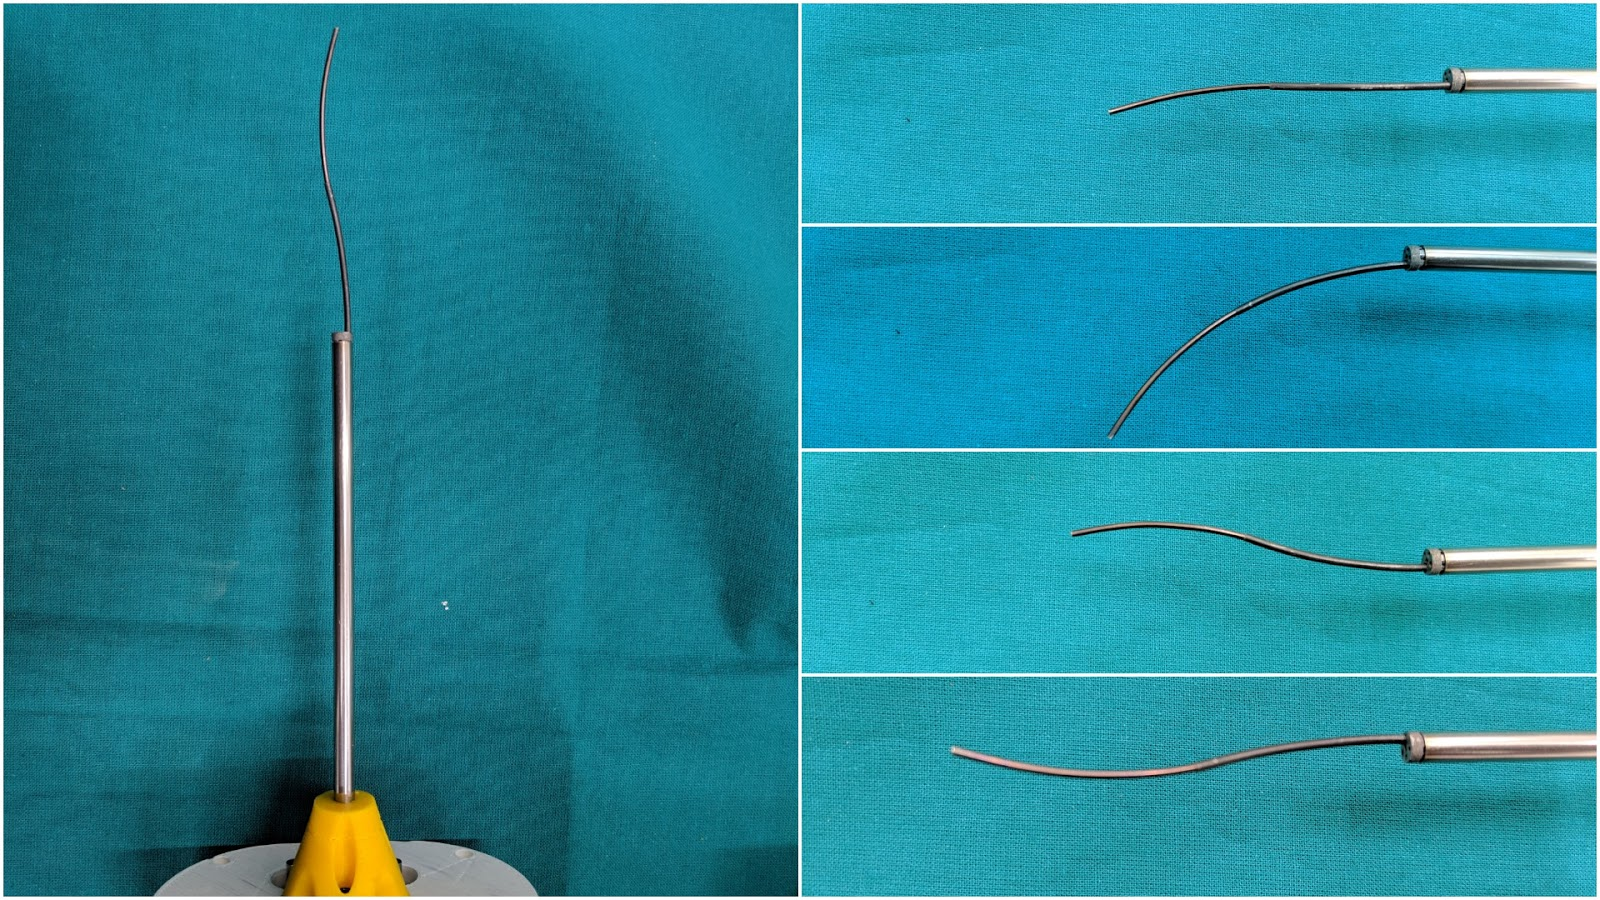
\includegraphics[scale=0.15]{fig1.jpg}
\caption{Curvilinear path of two tube concentric tube robot.}
\label{fig:1}
\end{figure}
Common modelling approaches of concentric tube robots are based on special Coserat rods for each tube undergoing bending and torsion that lead to no analytical solution for robots consisting of two tubes or more or for pre-curvature that varies with length \cite{Dupont2010}, \cite{Rucker2010}. Additional factors like friction and tube tolerances have have been investigated \cite{Lock2011} but are difficult to integrate because of the large computational load for modelling efforts. Inverse kinematics strategies applied are common approaches like numerical root finding \cite{Burgner2014} or differential inverse kinematics \cite{Dupont2010}. These strategies are slow and do not guarantee convergence with Coserat rod modelling. A model-free data driven approach (DDA) would be beneficial because of accuracy in real scenarios compared to current model-based inverse kinematics strategies. Furthermore, unlike neural network approaches that have been proposed \cite{Grassmann2018}, reinforcement learning can be trained in successively complex environments and eventually to a real environment by combining training parameters as shown in the Sim2Real \cite{OpenAI2018}. Reinforcement learning is then data efficient, if the cost of collecting real life data is high.

To our knowledge there have been no previous work using reinforcement learning for concentric tube robots. However, two DDA approaches have been proposed. The first approach \cite{Bergeles2015} uses simulated data to train a multi-layer perceptron (MLP) network for inverse kinematics of a 3 tube robot with one variable curvature section. The rotation configuration space is split into four quadrants resulting in an output of a single extension joint value per tube and 4 rotation joint values per tube. The correct joint tuple is selected by examining the least forward kinematics tip error. To avoid bias during training, extension values less than 30\% of the maximum extension value are ignored. The simulation accuracy results demonstrate Cartesian error is below 0.8mm running at 50 Hz in Matlab. The second approach \cite{Grassmann2018} also uses an MLP framework for inverse kinematics and focuses on hardware with a contribution with a novel joint space representation. The representation follows trigonometric joint representation used in other work with adaptions for concentric tube robots. The work defines a cylindrical form $\gamma_i$,
\begin{equation}
\gamma_i = \{ \gamma_{1,i}, \gamma_{2,i}, \gamma_{3,i} \} = \{ \cos(\alpha_i), \sin(\alpha_i), \beta_i \},\label{eqn:1}
\end{equation}
which describes the $i$ tube as a triplet. The rotatory joint $\alpha_i$ can be retrieved by
\begin{equation}
\alpha_i = \textnormal{atan2} \{ \gamma_{2,i}, \gamma_{1,i} \}. \label{eqn:2}
\end{equation}
The extension joint $\beta_i$ can be retrieved directly and has constraints
\begin{align}
0 \geq \beta_n \geq & \dots \geq \beta_2 \geq \beta_1, \label{eqn:3} \\
0 \leq L_n + \beta_n \leq & \dots \leq L_2 + \beta_2 \leq L_1 + \beta_1, \label{eqn:4}
\end{align}
where $n$ is the number of tubes. Another study \cite{Grassmann2019}, investigating various joint space representations confirmed that the cylindrical representation performs much better for MLP frameworks as compared a simple rotation and extension form. Hardware training and evaluation was done with a 3 tube concentric tube robot, the actuation error was $4.0$mm in translation and $8.3 ^{\circ}$ with 60,000 training samples. The cylindrical form and extension constraints are directly used as the joint representation for the reinforcement learning strategy applied in this work.

A major challenge of model-free reinforcement learning in continuous state and action spaces is exploration \cite{Nair2018}. An advantage of using an off-policy algorithm like deep deterministic policy gradient is the learned policy does not have to be the one used for training. In the first continuous control work \cite{Lillicrap2015}, Ornstein-Uhlenbeck was the noise process used for continuous problems but alternatives strategies have been found. The three main exploration methods are applied to model-free reinforcement learning are studied and results presented in this work. The exploration methods are Gaussian noise process, Ornstein-Uhlenbeck noise process and parameter noise. Applying the same exploration to different number of tubes is an indication that the policy can be generalized. Therefore, a focus is placed on finding exploration parameters that work from two to four tube dominant stiffness concentric tube robots.
\section{Methods}
Following the standard paradigm of reinforcement learning the inverse kinematics problem is formulated as a Markov Decision Process (MDP). The action, state and reward of the MDP model is detailed as follows.

\paragraph{State.} The state is a combination the cylindrical representation defined in equation \ref{eqn:1}, the current Cartesian end-effector position $g$ and the desired Cartesian end-effector position $\hat{g}$,
\begin{equation}
s = \left( \gamma_1, \gamma_2, \dots, \gamma_n, g, \hat{g} \right). \label{eqn:5}
\end{equation}

\paragraph{Action.} The action is a change in extension and rotation at one timestep with separate limits for rotation and extension. In DDPG, the agent can select any value in the continuous range in the limit interval.
\begin{equation}
a = \left( \Delta \alpha_1, \Delta \beta_1, \Delta \alpha_2, \Delta \beta_2,  \dots, \Delta \alpha_n, \Delta \beta_n \right). \label{eqn:6}
\end{equation}

\paragraph{Reward.} The reward is the scalar value returned by the environment as feedback to the agent from the chosen action at the current timestep. In \cite{andrychowicz2017hindsight} described how sparse rewards are more effective than dense rewards when using hindsight experience replay for continuous action environment. Moreover, dense rewards are difficult to shape to push the agent towards a desired behaviour. The error is
\begin{equation}
e = \sqrt{(g_x - \hat{g}_x)^2 + (g_y - \hat{g}_y)^2 + (g_z - \hat{g}_z)^2}. \label{eqn:7}
\end{equation}

The reward function can then be defined as
\begin{equation}
r =
  \left\{
    \begin{array}{l}
      \hphantom{-}0, \quad e \leq \delta \\
      -1, \quad \textnormal{otherwise},
    \end{array}
  \right. \label{eqn:8}
\end{equation}

where $\delta$ is the goal tolerance. The tolerance used in this work is 1 mm. An episode consists of a certain number of timesteps for the agent to interact with the environment, before a reset is initiated or the desired goal has been reached. The reward function is calculated at each timestep and is cumulative through the episode, therefore the agent is incentivized to use the fewest timesteps to the desired goal.

\subsection{Deep deterministic policy gradient and hindsight experience replay}
The model-free reinforcement learning algorithm chosen is deep deterministic policy gradient (DDPG) with hindsight experience replay (HER). Robotic control is a continuous state and action MDP, limiting the reinforcement learning algorithms compatible. \cite{andrychowicz2017hindsight} has shown successful control DDPG for dexterous and reaching tasks in robotics. The addition of HER adds more successful episodes during training, when without this replay strategy, successful episodes are sparse.

DDPG learns a policy or actor, $\mu(s)$, that predicts an action, $a$, given a state $s$. The technique also uses an action-value function or critic, $Q(s,a)$ which gives an expected utility for a given action when the system is at a particular state. Learning an optimal policy is grounded in using the policy function to output an action, and evaluate the action's utility with the action-value function. DDPG consists of 2 pairs of actor and critic artificial neural networks. The actor network and actor target network have weight parameters $\theta^\mu$ and $\theta^{\mu`}$ and critic network and critic target network have weight parameters $\theta^Q$ and $\theta^{Q`}$. To train off-policy, a replay buffer $R$ of finite size is stored in memory with experiences defined as a tuple $\left(s_t, a_t, r_t, s_{t+1}  \right)$. Iterating over a set number of episodes, the noise process and starting state is initialized. In each episode, there are three main sub-iterations. The first iteration collects samples by executing the exploratory policy through the environment for a given number of timesteps. The next iteration is storing the experiences in the replay buffer with HER. The last iteration is training the actor and critic networks. With $R$ initialized, training starts with sampling a random mini-batch of $N$ transitions $\left(s_i, a_i, r_i, s_{i+1}  \right)$ from $R$. The target at the $i$ sample for the loss function, $y_i$, is defined as
\begin{equation}
y_i = r_i + \gamma Q'(s_{i+1}, \mu'(s_{i+1} | \theta^{\mu'}) | \theta^{Q'}). \label{eqn:9}
\end{equation}
The loss function, $L$, for the critic network can then be formulated as
\begin{equation}
L = \frac{1}{N} \sum_i \left(y_i - Q(s_i, a_i | \theta^Q) \right)^2. \label{eqn:10}
\end{equation}
To train the policy network an objective function $J$ to maximize the expected return is defined as
\begin{equation}
J(\theta) = E[Q(s,a|\theta^Q|_{s=s_i, a_i = \mu(s_i| \theta^\mu)}]. \label{eqn:12}
\end{equation}
Taking the gradient of $J$ with respect to the policy parameters $\theta^\mu$, the update for the actor network is

\begin{equation}
\nabla_{\theta^\mu}J = \frac{1}{N} \sum_i \nabla_a Q(s,a|\theta^Q) |_{s=s_i,a=(s_i|\theta^\mu)} \nabla_{\theta^\mu} \mu(s|\theta^\mu)|_{s=s_i}. \label{eqn:13}
\end{equation}

Finally, the target networks are updated with
\begin{align}
    \theta^{Q'} &= \tau \theta^Q + (1 - \tau)\theta^{Q'} \\
    \theta^{Q'} &= \tau \theta^Q + (1 - \tau)\theta^{Q'}.    
\end{align}

Hindsight experience replay changes the way experiences are stored in the replay buffer. A trajectory with a desired goal is defined as a sequence of experiences in an episode,
\begin{equation}
\left( \left(s_0, a_0, r_0, s_1 \right), \left( s_1, a_1, r_1, s_2 \right), \dots, \left( s_{T-1}, a_{T-1}, r_{T-1}, s_T \right) \right).
\end{equation}
After each experience is stored in the replay buffer, additional experiences are created by iterating through the trajectory and appending the desired goal in the state. Recall in equation \ref{eqn:5}, the state is the cylindrical representation, achieved goal and desired goal. Specifically in the future HER strategy, iterating through the trajectory of the most recent episode, at each experience, $k$ future achieved goals, $g$, with their states, $s$, are sampled from the current experience till the end of the trajectory. With the future states, the achieved goal, $g$, is substituted as the desired goal, $\hat{g}$. Last, the new reward is calculated and stored in the replay buffer as a new experience.

The benefits of using HER is two fold. The first is in complex environments where successful trajectories are sparse, HER is able to add more successful trajectories and experiences. Second, as shown in [add citation], sparse rewards work better than dense rewards for policy gradient continuous state and action problems by eliminating the need for reward function shaping, a separate topic in reinforcement learning research.

\subsection{Gym Environment}
The kinematic model is the dominant stiffness model. Each tube is composed of a curved section and a final straight section at the end-effector. With $\alpha$ as the tube rotation relative to the base of the tube, $\kappa$ is the curvature of the tube and $L + \beta$ is the extension length. A transformation representing the curvature for a tube is defined as

\begin{equation}\label{curvature-transformation}
\begin{aligned}
^b \textbf{T}_i &=
\left[\begin{matrix}
  c^2_\alpha (c_{\kappa  \left(L+\beta\right)} - 1) + 1 & s_\alpha c_\alpha (c_{\kappa  \left(L+\beta\right)} - 1) \\
  s_\alpha c_\alpha (c_{\kappa  \left(L+\beta\right)} - 1) & c^2_\alpha (1 - c_{\kappa  \left(L+\beta\right)}) + c_{\kappa  \left(L+\beta\right)} \\
  c_{\phi} s_{\kappa  \left(L+\beta\right)} & s_{\phi} s_{\kappa  \left(L+\beta\right)} \\
  0 & 0
\end{matrix}\right.\\
&\qquad\qquad
\left.\begin{matrix}
  - c_\alpha s_{\kappa  \left(L+\beta\right)}  & \frac{L+\beta}{k} c_\alpha (c_{\kappa \left(L+\beta\right)} - 1) \\
  - s_\phi c_{\kappa \left(L+\beta\right)} & \frac{1}{k} s_\phi (c_{\kappa  \left(L+\beta\right)} - 1) \\
  c_{\kappa s} & \frac{1}{k} s_{\kappa  \left(L+\beta\right)} \\
  0 & 1
\end{matrix}\right],
\end{aligned}
\end{equation}
The straight section at the end-effector of the robot is a translation from the last tube with a length $l_{tip}$.
\begin{equation}
\label{straight-ee}
^n \textbf{T}_{ee} =
\left[\begin{matrix}
1 & 0 & 0 & 0 \\
0 & 1 & 0 & 0 \\
0 & 0 & 1 & l_{tip} \\
0 & 0 & 0 & 1 \\
\end{matrix}\right].
\end{equation}
For a single tube robot, the forward kinematics transform is
\begin{equation}
^b \textbf{T}_{ee} = ^b \textbf{T}_1 ^1 \textbf{T}_{ee}
\end{equation}
For a two tube robot, the curvature transform of the second tube is added.
\begin{equation}
^b \textbf{T}_{ee} = ^b \textbf{T}_1 ^1 \textbf{T}_2  ^2 \textbf{T}_{ee}
\end{equation}

To follow the standardization of reinforcement learning environments started by openAI gym, the one, two, three and four tube environments has been formulated as a openAI gym environment \cite{Brockman2016}. The main components are the reset, step and reward functions.

\paragraph{reset} The reset function resets the environment to begin a new episode and returns a first observation. A desired goal is determined by sampling from a uniform distribution of the joint states, and performing forward kinematics. The first episode has a specified initial joint position set to fully extended. Episodes after the first have the starting position of where the previous episode left off.

\paragraph{step} The step function performs a single timestep iteration of the environment given an action. The action is clipped to be within specified bounds. The action is added to the current joints of the robot and clipped and constrained by equation \ref{eqn:3} and \ref{eqn:4}. Appending the cylindrical form, achieved goal and desired goal, the state is formed. With the state, the reward can be computed. The environment has two termination conditions, if the Cartesian error $e$ is under the tolerance $\delta$ or the maximum number of time steps has been reached. If the environment has terminated, the reset function is called. The function returns, the new state, reward and terminal condition. 

\paragraph{reward} The reward function computes the reward at the current state. With the achieved and desired goal Cartesian points, equation is used to determine the error $e$. If the error is below the tolerance $\delta$, the reward is $0$. Otherwise the reward is $-1$. The function is defined in equation \ref{eqn:8}.

\subsection{Exploration}
There are three main exploration techniques found in model-free reinforcement learning. All three techniques add a noise to the action during training.

\paragraph{Zero-mean univariate and multivariate Gaussian noise}
Given a standard deviation, each action during training is perturbed by sampling a value from a zero-mean Gaussian distribution and adding it to the selected action.

\paragraph{Ornstein Uhlenbeck noise}
Ornstein-Uhlenbeck noise process was the original noise process in the DDPG paper. The noise is time dependant allowing to set a long-term mean $\mu$. The process moves towards $\mu$ with a given standard deviation $\sigma$ at a rate $\theta$ and current value $x_t$.
\begin{equation}
dx_t = \theta \left( \mu - x_t \right) d_t + \sigma d W_t
\end{equation}

\paragraph{Parameter noise}
Parameter noise adds noise directly to the policy network weights during training for exploration \cite{plappert2017parameter}. Zero mean multivariate Gaussian distribution of size equal to the parameter vector of the policy network is sampled and used to perturb the policy weights directly.

The study proposed is to investigate these exploration strategies in terms of accuracy and scalability with respect to number of tubes. To this end the proposed method of investigation is the following. With the 2 tube environment, a hyper-parameter search will be done for a exploration parameter, different to each strategy except for Ornstein-Uhlenbeck. Ornstein-Uhlenbeck will have a long-term mean of extension with an appropriate rate to last an episode with a standard deviation from the Gaussian approach. Once this parameter is found, training is done for 2,3 and 4 tube environments. Comparisons of accuracy, error and success during training can be done. Lastly, a measure of online adaptability will be done. With the 4-tube environment, if the tube parameters are changed dramatically, how long does it take for the exploration strategy to re-learn the correct policy.

\section{Testing and Results}
% For tables use
\begin{table}
% table caption is above the table
\caption{Hyperparameter Descriptions}
\label{tab:1}       % Give a unique label
% For LaTeX tables use
\begin{tabular}{lll}
\hline\noalign{\smallskip}
Hyperparameter & Description\\
\noalign{\smallskip}\hline\noalign{\smallskip}
timesteps & Total number of timesteps for training.\\
sampled\_goals & The number of artificial transitions to \\
& generate for each actual transition. \\
buffer\_size & The max number of transitions to store,\\
&  size of the replay buffer.\\
batch\_size &  The size of the batch for learning the policy.\\
gamma & Discount factor.\\
tau & Soft update coefficient for target network.\\
random\_exploration & Probability of taking a random action.\\
noise\_type & Type of noise to apply.\\
noise\_std & Standard deviation of specified noise type.\\
actor\_learning\_rate & The actor learning rate.\\
critic\_learning\_rate & The critic learning rate.\\
actor and critic network & Actor and critic network architecture.\\

\noalign{\smallskip}\hline
\end{tabular}
\end{table}

% For tables use
\begin{table}
% table caption is above the table
\caption{Static hyperparameters}
\label{tab:1} 
% For LaTeX tables use
\begin{tabular}{lllll}
\hline\noalign{\smallskip}
Hyperparameter  & Tube 1 \\
\noalign{\smallskip}\hline\noalign{\smallskip}
timesteps & 2e6 \\
sampled\_goals & 4 \\
buffer\_size & 10000 \\
batch\_size & 256 \\
gamma & 0.95 \\
tau & 0.001 \\
random\_exploration & 0.294 \\
noise\_type & normal \\
noise\_std & 0.35 \\
actor\_learning\_rate & 0.001 \\
critic\_learning\_rate & 0.001 \\
actor and critic network & [128, 128, 128] \\

\noalign{\smallskip}\hline
\end{tabular}
\end{table}

% For tables use
\begin{table}
% table caption is above the table
\caption{Concentric tube robot environment parameter description}
\label{tab:2}       % Give a unique label
% For LaTeX tables use
\begin{tabular}{lll}
\hline\noalign{\smallskip}
Parameter & Description & Units\\
\noalign{\smallskip}\hline\noalign{\smallskip}
k & Curvature of each tube. & m$^{-1}$ \\
l\_tip & Length of end-effector straight section. & m \\
tube\_length & Length of each tube. & m\\
tube\_rotation\_limits & Range of orientation for rotation & $^\circ$ \\
action\_length\_limit & Largest change in length in single timestep. & m \\
action\_rotation\_limit & Largest change in length in single timestep. & $^\circ$ \\
goal\_tolerance & Tolerance to desired goal for a successful episode. & m \\

\noalign{\smallskip}\hline
\end{tabular}
\end{table}

% For tables use
\begin{table}
% table caption is above the table
\caption{Concentric tube robot environment parameters}
\label{tab:2}       % Give a unique label
% For LaTeX tables use
\begin{tabular}{lllll}
\hline\noalign{\smallskip}
Parameter & 1-Tube & 2-Tube & 3-Tube & 4-Tube\\
\noalign{\smallskip}\hline\noalign{\smallskip}
k & 25.0 & 25.0, 20.0 & 15.0 & 10.0\\
l\_tip  & 0.007 & 0.007 & 0.007 & 0.007\\
tube\_length & 0.10 & 0.15, & 0.12, 0.07, & 0.15, 0.10, \\
& & 0.10 & 0.04 & 0.05, 0.025 \\
tube\_rotation\_limits  & -180$^\circ$,  & -180$^\circ$, & -180$^\circ$, & -180$^\circ$,\\
& 180$^\circ$ & 180$^\circ$ & 180$^\circ$ & 180$^\circ$\\
action\_length\_limit & -0.0001, 0.0001 & -0.0001, & -0.0001, & -0.0001, \\
& 0.0001 & 0.0001 & 0.0001 & 0.0001 \\
goal\_tolerance & 0.001 & 0.001 & 0.001 & 0.001\\

\noalign{\smallskip}\hline
\end{tabular}
\end{table}


\begin{itemize}
    \item Show table of static hyperparameters
    \item Table of dynamic hyperparameters
    \item Tests:
    \begin{itemize}
        \item Multivariate Gaussian noise of different extension stds on different tubes
        \item Hyperparameter search for parameter noise value on different tubes
        \item OU noise with similar Gaussian noise stds on different tubes
        \item Take best noise on each tube, do a online training test
    \end{itemize}
    \item Hopefully conclusion is either OU or Gaussian works best and can be used even online.
    \item Future work is adapting best noise parameter for realisitic models since exploration is somewhat understood.

\end{itemize}

\section{Conclusion}

%\begin{acknowledgements}
%If you'd like to thank anyone, place your comments here
%and remove the percent signs.
%\end{acknowledgements}


% Authors must disclose all relationships or interests that 
% could have direct or potential influence or impart bias on 
% the work: 
%
% \section*{Conflict of interest}
%
% The authors declare that they have no conflict of interest.


% BibTeX users please use one of
%\bibliographystyle{spbasic}      % basic style, author-year citations
%\bibliographystyle{spmpsci}      % mathematics and physical sciences
\bibliographystyle{spphys}       % APS-like style for physics
\bibliography{refs}   % name your BibTeX data base

% Non-BibTeX users please use
%\begin{thebibliography}{}
%
% and use \bibitem to create references. Consult the Instructions
% for authors for reference list style.
%
% \bibitem{RefJ}
% Format for Journal Reference
% Author, Article title, Journal, Volume, page numbers (year)
% Format for books
% \bibitem{RefB}
% Author, Book title, page numbers. Publisher, place (year)
% etc
% \end{thebibliography}

\end{document}
% end of file template.tex

